\documentclass[10pt,review]{elsarticle}
\usepackage{hyperref}
\usepackage[margin=1in]{geometry}
\usepackage{graphicx}
\usepackage{amsmath}
\usepackage{placeins}
\usepackage{comment}
\usepackage{gensymb}
\usepackage{lineno}
\usepackage{color}
\usepackage{cleveref}


%\journal{Journal of Nuclear Materials}
\bibliographystyle{elsarticle-num}

\begin{document}

\begin{frontmatter}
\title{Radiation driven diffusion in $\gamma$U-Mo}

\author[ncsu,inl]{Benjamin Beeler\corref{qwe}}
\cortext[qwe]{Corresponding author}
\ead{benjamin.beeler@inl.gov}
\author[lanl]{Michael W.D. Cooper}
\author[anl]{Zhi-Gang Mei}
\author[inl]{Daniel Schwen}
\author[wisc,inl]{Yongfeng Zhang}
\address[ncsu]{North Carolina State University, Raleigh, NC 27695}
\address[inl]{Idaho National Laboratory, Idaho Falls, ID 83415}
\address[lanl]{Los Alamos National Laboratory, Los Alamos, NM 87545}
\address[anl]{Argonne National Laboratory, Lemont, IL 60439}
\address[wisc]{University of Wisconsin-Madison, Madison, WI 53715}

\begin{abstract}
Under the United States High-Performance Research Reactor (HPRR) program, a number of research reactors are planned to undergo a conversion to a U-Mo monolithic fuel design. Both experimental and computational campaigns are underway to ensure the stable and predictable behavior of this fuel type under operation. The accurate prediction of fuel evolution under irradiation requires implementation of correct thermodynamic and kinetic properties into mesoscale and continuum level fuel performance modeling codes. One such property where there exists incomplete data is the diffusion of relevant species under irradiation. Fuel performance swelling predictions rely on an accurate representation of diffusion in order to determine the rate of fission gas swelling and the local microstructural evolution. In this work, we present molecular dynamics simulations combined with rate theory calculations to determine the radiation enhanced diffusion of U and Mo as a function of temperature and fission rate. In combination with previous studies on intrinsic diffusion and radiation driven diffusion in U-Mo alloys, this study completes the multi-component diffusional picture for the U-Mo system. Fuel performance simulations are conducted to illustrate the impact of such fundamental property collection. 

\end{abstract}
\end{frontmatter}

\linenumbers
\modulolinenumbers[5]

\section{Introduction}

\begin{comment}
High power research reactors typically employ a highly enriched uranium (HEU) dispersion type fuel. The United States High-Performance Research Reactor (USHPRR) program targets replacing current HEU fuel in research reactors with low enriched uranium (LEU) fuel \cite{snelgrove1997}. In order to achieve a reduced enrichment in these fuel types, there is the requirement for increased uranium density. The fuel design being pursued under the USHPRR program is a uranium-molybdenum (U-Mo) monolithic foil, with a zirconium (Zr) diffusion barrier in aluminum (Al) cladding.

An issue with U-Mo monolithic fuel is the large amount of swelling that takes place during operation \cite{hofman1997}. Such swelling needs to be stable and predictable up to high fission densities. Research reactor fuel types based on U-Mo are unique in their design to stably retain fission gases to high fission densities, and as such there is a relatively high content of fission gas and of fission gas bubbles within the fuel matrix. The importance of swelling in addition to the unique fuel environment has led to a variety of experimental studies characterizing the swelling behavior in U-Mo fuels \cite{rest2009, kim_anl08, meyer2002, kim2013}, which has led to the development of a swelling correlation as a function of fission density from Argonne National Laboratory (ANL) \cite{kim2011} and Idaho National Laboratory (INL) \cite{umo_prelim_report2017}. A 2015 post-irradiation examination (PIE) report \cite{afip6report} from Williams, et al. showed higher swelling in U-10Mo (alloy composition is provided in weight percent unless otherwise noted) fuels at fission densities much lower than previously observed. This accelerated fuel swelling behavior could lead to early fuel failure and was not captured by the ANL correlation. As such, a more mechanistic fuel swelling model is needed in order to predict swelling behavior of U-Mo fuels under both typical operating conditions, as well as transients, accident scenarios and different reactor environments.

Recently, substantial effort has been made on mesoscale models to describe the swelling behavior of U-Mo fuels \cite{liang2018, liang2018a, liang2017, liang2016, ye2018, hu2017a, hu2016, hu2016a}. These models rely on phase-field and/or rate theory descriptions of material systems in order to model swelling on realistic timescales on a microstructural level. These simulation methodologies include a number of parameters that are either fit to limited experimental data, calculated from lower length scale modeling methodologies, or assumed based on other material systems. One such assumption is the diffusion of species at low temperature. Research reactor fuels operate at relatively low temperatures, within a range of 150\degree C to 350\degree C. Intrinsic, thermal diffusion is relatively limited at these temperatures and no such experimental data on diffusive behavior in this temperature range exists. 

A number of high temperature experimental studies have been conducted on interdiffusion, tracer diffusion and self-diffusion in the U-Mo system. Adda, et al. determined the interdiffusion coefficient of U-Mo from 1123 K to 1323 K and subsequently determined the self-diffusion coefficient of uranium with 10 atomic percent Mo \cite{adda1962}.  Lundberg determined interdiffusion coefficients from 1400 K to 1525 K for a range of high Mo content systems (higher than U-10Mo) \cite{lundberg1989}. Huang, et al. calculated interdiffusion and intrinsic diffusion of U-Mo alloys from 923 K to 1273 K via diffusion couples \cite{huang2013}. All of these experimental studies agree that in U-rich U-Mo alloys, U diffuses more rapidly than Mo and that the interdiffusion coefficient is reduced with the addition of Mo. However, none of these studies investigated low temperature systems due to the difficulties in obtaining data due to reduced intrinsic diffusion of species at low temperatures. Thus, the diffusion data are often extrapolated from high temperature systems to low temperature as a means of estimation. Additionally, there are no experimental studies of fission gas diffusion in U-Mo alloys. 

For the study of self- and fission gas diffusion in UO$_2$, the nuclear fuel type typically utilized in commercial reactors in the U.S., the total diffusion coefficient is typically broken down into three component parts: 1) intrinsic diffusion (D$_1$), 2) radiation enhanced diffusion (D$_2$), and 3) radiation driven diffusion (D$_3$). Each of these constituent parts is dominant in a given temperature regime, as was initially discussed by Turnbull \cite{turnbull1982} and computationally investigated by Andersson, et al. \cite{andersson2014} and Cooper, et al. \cite{cooper2016}, and others \cite{matthews_cluster_2019, perriot_atomistic_2019, wormald2015, martin2009}. Given the low operating temperatures of research reactors, it is expected that radiation driven diffusion will be a critical component of the total diffusion. No experimental or computational studies have been performed to investigate radiation driven diffusion in U-Mo or U-Mo-Xe systems.

In this work, molecular dynamics simulations are performed to determine the radiation driven diffusion of U, Mo and Xe in U-Mo nuclear fuels. Diffusion coefficients for each species are determined over a range of temperatures and compositions. Updated diffusion coefficients are presented that are applicable under irradiation that incorporate both intrinsic and radiation driven diffusion. 

\end{comment}

\section{Computational Details}

The rate of change of defect concentrations with time can be described by equation \ref{eq:1} and \ref{eq:2}

\begin{equation}
\label{eq:1}
\frac{dC_v}{dt} = \epsilon \dot F - K_{iv}C_iC_v - k^2_{vs}D_vC_v
\end{equation}
\begin{equation}
\label{eq:2}
\frac{dC_i}{dt} = \epsilon \dot F - K_{iv}C_iC_v - k^2_{is}D_iC_i
\end{equation}

where $\dot F$ is the fission rate, $\epsilon$ is the defect production, K is the recombination constant of vacancies and interstitials, k$^2$ is the sink strength of grain boundaries, and D is the diffusion coefficient. The subscripts \textit{i}, \textit{v}, and \textit{s} denote interstitial, vacancy, and sink, respectively. In this case, sinks are restricted to grain boundaries. The defect production is calculated from the arc-dpa model \cite{arcdpa}, which is a modification of the NRT model for calculating displacements that also includes recombination. The number of defects generated is described by the arc-dpa model as:

\begin{equation}
\label{eq:3}
N_d = \frac{0.8T_d}{2E_d}\zeta(T_d)
\end{equation}

where T$_d$ is the damage energy, E$_d$ is the displacement energy, and $\zeta$ is the arc-dpa efficiency function. The magnitude of E$_d$ and $\zeta$ for $\gamma$-UMo is not well known, but can potentially be determined from molecular dynamics or from experiments. Given that such studies are beyond the scope of this work, reasonable approximations are made for the displacement energy of 60 eV, based upon molecular dynamics simulations in $\gamma$U \cite{beeler_Ed}, and for the efficiency of 0.25, which is approximately the same as bcc Fe \cite{arcdpa}. The damage energy is taken as the kinetic energy of the fission fragments produced from a fission reaction (approximately 170 MeV), and reduced to account for electronic energy losses. It is assumed that only ballistic effects are generating Frenkel pairs in this work. The electronic energy losses have been previously calculated by Beeler, et al. \cite{beeler_rad} to be 95\%, thus the damage energy here is taken as 8.5 MeV. This yields a number of defects per fission in $\gamma$-UMo of approximately 14,000. Any bias towards interstitials or vacancies in the defect production process is neglected, assuming that an equal number of both types of defects are generated. 

Two sets of molecular dynamics simulations are performed to calculate rate coefficients: a) point defect diffusion, and b) defect evolution in a bulk system. Molecular dynamics simulations are performed utilizing the LAMMPS \cite{plimpton1995} software package and a U-Mo-Xe embedded atom method (EAM) interatomic potential from Smirnova \cite{smirnovaUMo}. For short atomic distances, this interatomic potential was splined to a ZBL \cite{zbl} via LAMMPS with spline cutoffs of 1 {\AA} and 2 {\AA}. This potential has been shown to reasonably predict a number of properties of $\gamma$-UMo, while also being the only ternary interatomic potential capable of describing the U-Mo-Xe system. 

To determine diffusion coefficients of a single vacancy or interstitial, a system of 2000 atoms (10x10x10 unit cells) was generated in the body-centered cubic (bcc) structure with an atomic composition of 23\% Mo, corresponding to U-10Mo (weight percent). A single defect is randomly generated and the system is equilibrated at a given temperature in an NPT ensemble for 50 ps. Subsequently, the ensemble is switched to an NVT and the system is allowed to evolve for another 100 ns, over which the mean-squared displacement (msd) as a function of time is analyzed. The Nose-Hoover thermostat and barostat as implemented in LAMMPS is utilized, with damping parameters each of 0.1. The msd as a function of time is fit to a linear function and utilized in the Einstein equation (D=msd/6t) in order to calculated the diffusion coefficient for a given temperature. Data for temperatures from 600 K up to 1200 K are obtained, and the entire dataset is fit to an Arrhenius equation, allowing for the determination of the diffusion coefficient prefactor and migration energy for a given defect type. 

In order to determine the rate coefficient of recombination (K$_{iv}$), a supercell of 128000 atoms (40x40x40 unit cells) was generated in the body-centered cubic (bcc) structure with an atomic composition of 23\% Mo at the equilibrium lattice constant for a given temperature. Fifty vacancies are removed and fifty interstitials are inserted, ensuring that the distance between individual defects is at least 4$\times$a0, where a0 is the lattice constant. The system is equilibrated for 20000 timesteps with a variable timestep such that a maximum distance for an atom to move in one timestep is 5 fm, in order to perform a constrained relaxation of the defects. Subsequently the system is evolved for 10 ns with a timestep of 1 fs, tracking the number of Frenkel pairs as a function of time via the Voronoi occupation methodology within LAMMPS. Without production and GB absorption, solving equations \ref{eq:1} and \ref{eq:2} leads to C = C$_0$/(C$_0$K$_{iv}$t +1) for vacancies and interstitials, where C$_0$ is the initial concentration. For a given temperature, the number of defects as a function of time can be fit to this relationship. 

In classical rate theory, the GBs are constant sinks and their strength k$^2$ is estimated as 15/L$^2$ (L is the grain size, in unit of nm here) for GBs with a regular pattern, and is identical for both interstitials and vacancies. This assumption is utilized here as a first approximation, and completes the parametrization of the rate theory equations.

Given a steady-state concentration of defects under irradiation, the radiation enhanced diffusion coefficient can be expressed as:

\begin{equation}
\label{eq:4}
D_{red} = D^{th}_iC^{irr}_i + D^{th}_vC^{irr}_v
\end{equation}

where D$_{th}$ is the thermal (intrinsic) diffusion coefficient, C$_{irr}$ is the equilibrium concentration of defects under irradiation, and subscripts \textit{i} and textit{v} denote interstitials and vacancies. Utilizing both experimental diffusional investigations and previously computational studies, the total diffusivity can then be taken as the summation of the intrinsic diffusion, D$_1$, the radiation driven diffusion, D$_3$, and the radiation enhanced diffusion, D$_2$.


\section{Results}

\begin{comment}

\subsection{Radiation driven diffusion of different elements}



\subsection{Effect of composition}

In U-Mo monolithic fuel, there can exist compositional variation due to processing procedures and the thermodynamics of interfaces and second phases present in the fuel. Such compositional variation can have an effect on properties, including the melting point and defect formation energies. As such, it needs to be understood if compositional variation will affect radiation driven diffusion. Compositions of U-4Mo, U-7Mo, U-10Mo and U-15Mo are investigated (compositions in weight percent), with the results at 500 K summarized in Fig. \ref{fig:A_comp} and table \ref{tab1}. There exists a clear trend of increasing diffusion (linearly proportional to $A$ from equation \ref{eq:2}) with decreasing Mo content. The most rapid radiation driven diffusion occurs for the U-4Mo system and the most sluggish diffusion is present for the U-15Mo system. This can largely be explained by the phenomenon of localized melting in the cascade core. For two similar systems and one system with a lower melting point, one would expect a greater extent of localized melting due to a cascade with a given PKA energy in the system with a lower melting point. The brief liquid-like behavior can accelerate diffusion due to ballistic mixing. From the phase diagram of U-Mo we see that alloying with Mo increases the melting point of the bcc phase of U \cite{umo_handbook}, in that a lower Mo content yields a lower melting point. That the interatomic potential captured this behavior was verified via the evolution of a two-dimensional solid/liquid interface, which found the melting point varied from approximately 1600 K for U-15Mo to 1500 K for U-4Mo. The extent of the differences in diffusion with respect to composition are more pronounced than the effects of temperature in Fig. \ref{fig:msdT}, but are still less than one order of magnitude. Thus, although there is a distinguishable difference in diffusion as a function of composition, utilizing the diffusion for U-10Mo for all Mo compositions from 7-15 weight percent is a valid assumption. 

\begin{figure}[h]
 \centering
 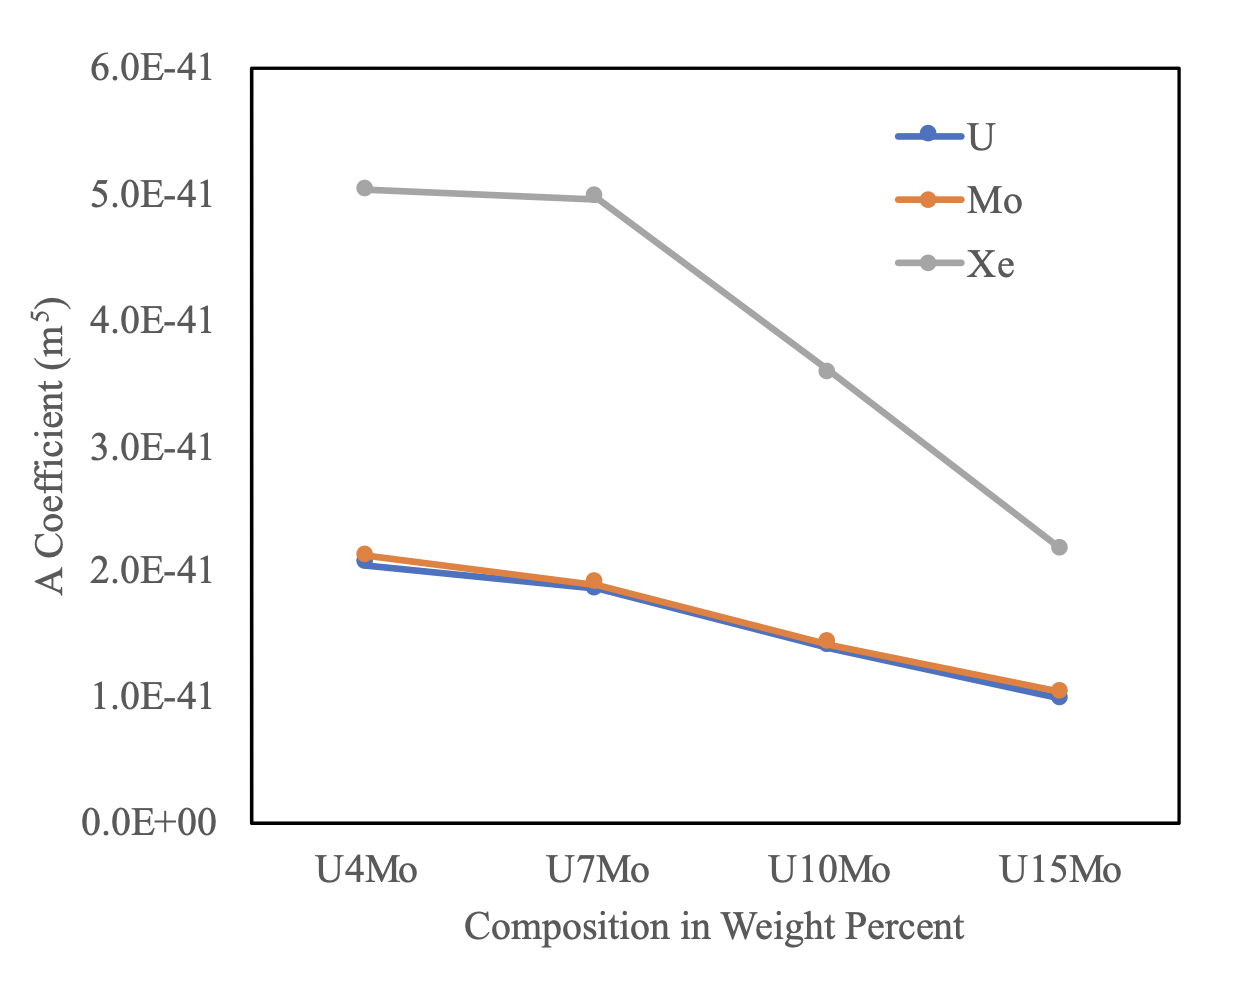
\includegraphics[width=0.7\textwidth]{7_A_comp.png} 
 \caption{The mean squared displacement as a function of energy deposition at four different compositions for U, Mo and Xe at 500 K.}
 \label{fig:A_comp}
\end{figure}

\begin{table}[h!]
\caption{The \textit{A} coefficient from equation \ref{eq:2} for different U-Mo alloy compositions at 500 K. }
\label{tab1}
\begin{center}
\begin{tabular}{|c|c|c|c|c|}
     \hline
Element & U-4Mo & U-7Mo & U-10Mo & U-15Mo  \\
\hline
U & 2.90E-41 & 2.62E-41 &  1.97E-41 & 1.39E-41 \\
Mo & 3.00E-41 & 2.69E-41 & 2.01E-41 & 1.46E-41 \\
Xe & 7.13E-41 &  7.03E-41 & 5.07E-41 & 3.07E-41  \\
 \hline
\end{tabular}
\end{center}
\label{default}
\end{table}%


\subsection{Updated diffusion coefficients}

Given the data in table \ref{tab1} and assuming that values for U-10Mo at 500 K are representative for all U-Mo systems in this study, new diffusion coefficients that incorporate both intrinsic and radiation driven diffusion can be presented. Fitting to the intrinsic diffusion data from Huang \cite{huang2013} yields diffusion coefficients of (1.28$\times$10$^{-5}$)$\times$exp(-1.76/kT) for uranium and (1.62$\times$10$^{-5}$)$\times$exp(-1.97/kT) for molybdenum (units in m$^2$/s and eV for the prefactor and activation energy, respectively). The intrinsic diffusion coefficient for Xe in U-Mo is unknown, but is commonly assumed to be approximately four orders of magnitude lower than the intrinsic diffusion of uranium \cite{hu2016a, ushprr17, ushprr18}, and this assumption is utilized here. It should be emphasized that these experimental data were collected at high temperature, and the Arrhenius fits to the data are being extrapolated to low temperatures to generate approximate intrinsic diffusion at reactor-relevant temperatures. This information is incorporated into \cref{eq3,eq4,eq5}, and assuming a fission rate of 5$\times$10$^{20}$ fiss/m$^3$-s \cite{ushprr17, ushprr18}, the total diffusion is shown in Fig. \ref{fig:totaldiff} for U, Mo and Xe as a function of temperature. 

\begin{align}
 D_U = (1.28\times10^{-5})\times exp(-1.76/kT) + 1.97\times10^{-41} \times \dot{F} \label{eq3}  \\
 D_{Mo} = (1.62\times10^{-5})\times exp(-1.97/kT) + 2.01\times10^{-41} \times \dot{F} \label{eq4} \\
 D_{Xe} = (1.28\times10^{-9})\times exp(-1.76/kT) + 5.07\times10^{-41} \times \dot{F} \label{eq5}
\end{align}

\begin{figure}[h]
 \centering
 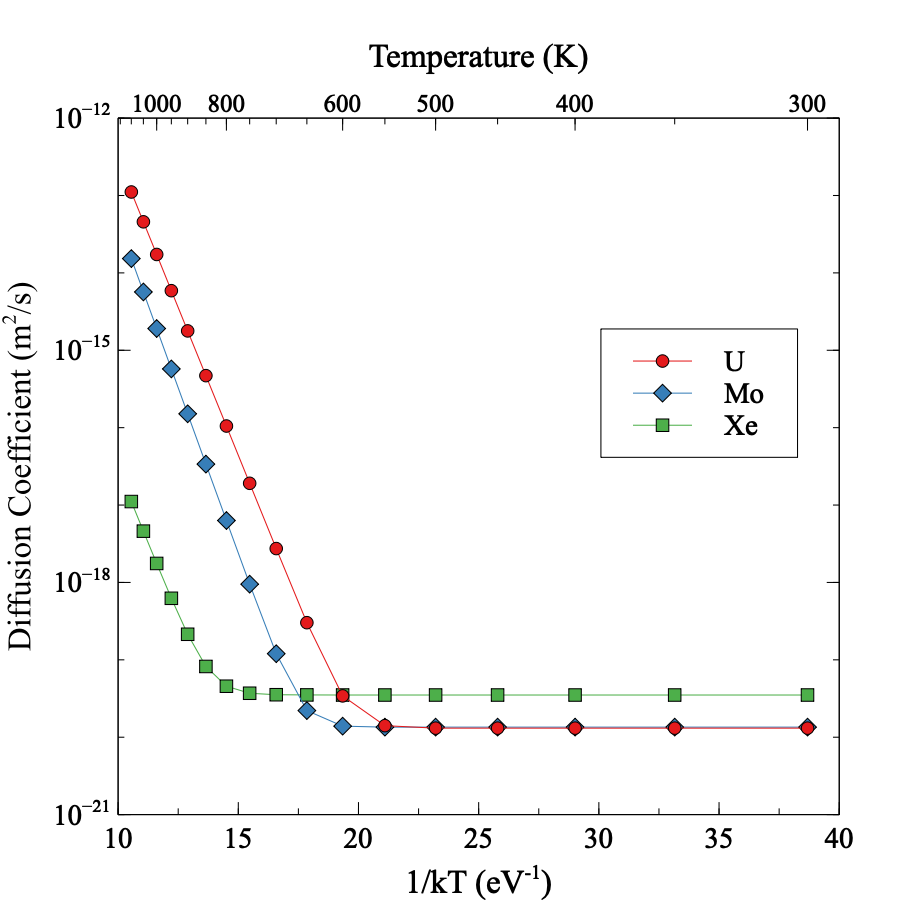
\includegraphics[width=0.8\textwidth]{8_total_diff.png} 
 \caption{The diffusion of U, Mo and Xe in U-Mo alloys as a function of temperature, including effects of both intrinsic and radiation driven diffusion. This graph assumes a fission rate of 5$\times$10$^{20}$ fiss/m$^3$-s.}
 \label{fig:totaldiff}
\end{figure}

There exists a transition for each species from intrinsic to radiation driven diffusion at a given temperature. The temperature at which each transition occurs is dependent upon the individual diffusive properties of each species (and the fission rate), where in this case the transition for U occurs at 600 K, Mo at 650 K, and Xe at 800 K. This means that below these transition temperatures, radiation driven diffusion is dominant compared to intrinsic diffusion. It should be emphasized that relevant temperature range of interest for U-Mo monolithic fuel in research reactors is from approximately 400 - 600 K. Thus, it is expected that intrinsic diffusion is not the dominant diffusion mechanism in this fuel in-reactor.

It should additionally be noted that radiated enhanced diffusion (D$_2$) is not calculated in this work and is unknown. It is entirely possible that D$_2$ is the dominant diffusion mechanism over some of all of the temperature regime of interest. However, given that it is unknown, the most complete diffusion data for the U-Mo-Xe system is as described in \cref{eq3,eq4,eq5}. Exclusion of D$_3$, and a reliance on only D$_1$, would result in a very significant underestimate of diffusivity at reactor operating temperatures. In the future, this research will extend towards investigating radiation enhanced diffusion in order to obtain the full characterization of diffusive behavior in U-Mo fuels. 

\FloatBarrier


\end{comment}


\section{Conclusions}

In this work, molecular dynamics simulations were performed to determine the radiation driven diffusion of U, Mo and Xe in U-Mo nuclear fuels. Diffusion coefficients for each species were determined and their variance as a function of composition and temperature was analyzed. Updated diffusion coefficients were presented that are applicable under irradiation that incorporate both intrinsic and radiation driven diffusion. This work demonstrates that at temperatures relevant to U-Mo research reactors, it is critical to account for radiation driven diffusion, as this is the dominant mode of diffusion when compared to intrinsic diffusion. The data generated in this manuscript can directly be incorporated into mesoscale and continuum fuel evolution and fuel performance models that describe fission gas and point defect behavior in U-Mo fuels. Finally, this work points to the possibility of an important role of radiation enhanced diffusion in U-Mo-Xe systems, and as such this will be the topic of future investigation. 


\section{Acknowledgement}
This work was supported by the U.S. Department of Energy, Office of Material Management and Minimization, National Nuclear Security Administration, under DOE-NE Idaho Operations Office Contract DE-AC07-05ID14517. This work was also supported by the U.S. Department of Energy, Office of Nuclear Energy, Nuclear Energy Advanced Modeling and Simulation (NEAMS) Program. This manuscript has been authored by Battelle Energy Alliance, LLC with the U.S. Department of Energy. The publisher, by accepting the article for publication, acknowledges that the U.S. Government retains a nonexclusive, paid-up, irrevocable, worldwide license to publish or reproduce the published form of this manuscript, or allow others to do so, for U.S. Government purposes. Los Alamos National Laboratory, an affirmative action/equal opportunity employer, is operated by Los Alamos National Security, LLC, for the National Nuclear Security Administration of the U.S. Department of Energy under Contract No. DE-AC52-06NA25396. This research made use of the resources of the High Performance Computing Center at Idaho National Laboratory, which is supported by the Office of Nuclear Energy of the U.S. Department of Energy and the Nuclear Science User Facilities.

\section{References}

\bibliography{MARMOTbib}


\end{document} 
